
\subsection{Elements}

Having concluded our survey of material and philosophical history, we are ready to develop the theory.
Our goal will be to develop a representation of subjective experience that is amenable to formal analysis.

Central to this theory will be the notion of pairwise preferences, which we have attempted to justify as a valid, yet formal, representation of subjective experience.

Before we can assess preference, we must establish some criterion to evaluate preferences against.
Among the same candidate set of answers, different questions can easily lead to different preferences.
For example, ranging over the items in your fridge, the questions \say{what to eat for breakfast} and \say{what to eat for dinner} will (likely) lead to different preferences among the same set of options.

\bigskip

We define questions with maximum generality, considering a general \say{question object} $Q$.
The representation of $Q$ is intentionally unspecified; the specific from of $Q$ will affect only the interpretation of the results, not the underlying theory.

We anticipate that $Q$ will often be represented via a string of characters (as in the fridge example).
However, $Q$ could be an image, a sound, an equation, or some new object yet unimagined.

\bigskip

In order to ask questions, we need candidate answers.
These candidate answers are members of an \textit{answer set} $A$.
As with the question object $Q$, the specific representation of the elements of $A$ are intentionally unspecified.

\bigskip

In order to represent subjective experience, we need an entity capable of subjective experience.
Discussions of subjectivity inevitably involve discussions of the notoriously elusive topic consciousness.
While the exact nature of consciousness is not known, researchers generally agree that conscious experience is attributed to discrete entities: as an entity I have an experience of consciousness that is separate from the experiences of other entities.
 
To resolve group preferences, we need a set of such discrete entities.
This set of entities is denoted $E$.
Unsurprisingly and in the spirit of this exposition, we leave the specific nature of these entities intentionally unspecified.
We anticipate that these entities will often be people. Later in this work we will introduce potential new directions for this theory, for which we may want to define these entities differently. Specifically, we will see how the problem of defining entities can be understood as selecting an \say{access policy}, the choice of which will shape the interpretation of the results.

\bigskip

Having introduced questions, answers, and entities, we are ready to introduce the \say{socrata}, conceived of as a basic unit of subjective experience. As the name suggests, a socrata represents an \textit{answer to a question}. Socrata have five components:

\begin{enumerate}
	\item A question object $Q$.
	\item An entity $e \in E$.
	\item A candidate answer $\alpha \in A$.
	\item A second candidate answer $\beta \in A$.
	\item The preference $p \in \{-1, 1\}$, where $1$ corresponds to preferring $\alpha$.
\end{enumerate}

It is not immediately obvious how we might operate on this representation. Recalling that preferences are only defined relative to a question $Q$, we can make $Q$ implicit. Further, for the moment let us assume that we are interested only in the preferences of a single entity $e$.

Now, we see that the salient attributes of a socrata are the two options $\alpha, \beta$, as well as the preference $p$. If we imagine $\alpha$ and $\beta$ as nodes, then $p$ can be represented as a directed edge between the two. Specifically, we create an edge $(\beta, \alpha)$ if $p = -1$ or $(\alpha, \beta)$ if $p = 1$ (the edge flows from loser to winner):

\begin{center}
\begin{tikzpicture}[node distance=3cm]
\node [roundnode] (a) {$\alpha$};
\node [roundnode] (b) [right of=a] {$\beta$};
\draw[ultra thick, <-] (a) -- (b);
\end{tikzpicture}
\end{center}

This graphical representation is desirable, as it suggests a natural way of aggregating socrata. Imagine we have $A = \{a, b, c, d\}$. The entity generates the following socrata:

\begin{center}

\socrata{a}{b}

\socrata{a}{c}

\socrata{b}{d}

\socrata{c}{b}

\end{center}

We can aggregate these socrata into the following \textit{socrata graph} $S$:

\begin{center}
\begin{tikzpicture}[node distance=3cm]
\node [roundnode] (a) {a};
\node [roundnode] (b) [right of=a] {b};
\node [roundnode] (c) [below of=a] {c};
\node [roundnode] (d) [right of=c] {d};
\draw[ultra thick, ->] (b) -- (a);
\draw[ultra thick, ->] (c) -- (a);
\draw[ultra thick, ->] (d) -- (b);
\draw[ultra thick, ->] (b) -- (c);
\end{tikzpicture}
\end{center}

Aggregating socrata across multiple entities presents little difficulty.
If we have entity $\alpha$ generating the following (an ordered preference of $a, b, c$):

\begin{center}

\socrata{a}{b}

\socrata{a}{c}

\socrata{b}{c}

\end{center}

And entity $\beta$ generating the following (an ordered preference of $a, c, b$):

\begin{center}

\socrata{a}{b}

\socrata{a}{c}

\socrata{c}{b}

\end{center}


We can assign each socrata a weight of 1 and combine the edges.
Parallel edges sum, while antiparallel edges cancel:

\begin{center}
\begin{tikzpicture}[node distance=3cm]
\node [roundnode] (a) {a};
\node [roundnode] (b) [right of=a] {b};
\node [roundnode] (c) [below of=a] {c};
\draw[ultra thick, ->] (b) -- node[auto] {2} (a);
\draw[ultra thick, ->] (c) -- node[auto] {2} (a);
\end{tikzpicture}
\end{center}

We denote this weight $w(u,v) \in \mathbb{N}^+$.

It is instructive to see what occurs in the instance of two entities with opposing preferences.
Say we $\alpha$ with preferences $(a, b, c)$, and $\beta$ with preferences $(c, b, a)$.
We might say we could resolve this by selecting $b$, as this seems the mutually-agreeable option.

Is this principled?
Selecting $b$ would cause both entities to have their second preference, a forfeiting of one item each.
Selecting $a$ or $c$, on the other hand, would cause one entity to have its first preference, and the other third --- a forfeiture of two items.
In a sense, this pair of opposing preferences render all answers equal.

Observe what happens in the corresponding socrata graph:

\begin{center}
\begin{tikzpicture}[node distance=3cm]
\node [roundnode] (a) {a};
\node [roundnode] (b) [right of=a] {b};
\node [roundnode] (c) [below of=a] {c};
\draw[ultra thick, -] (b) -- node[auto] {1-1} (a);
\draw[ultra thick, -] (c) -- node[auto] {1-1} (b);
\draw[ultra thick, -] (a) -- node[auto] {1-1} (c);
\end{tikzpicture}
\end{center}

\begin{center}
\begin{tikzpicture}[node distance=3cm]
\node [roundnode] (a) {a};
\node [roundnode] (b) [right of=a] {b};
\node [roundnode] (c) [below of=a] {c};
\end{tikzpicture}
\end{center}

The answers are disconnected; we interpret as an absence of preference.

\bigskip

\textit{A note on method:} we have been very intentional in our avoidance of assigning numerical value to subjective preference.
For an \textit{individual} entity (with an emphasis on the literal meaning of \say{individual} as non-divisible), preference is non-numeric.
Populations have magnitudes, however, and so we can comfortably reason in terms of sums and ratios when considering groups of entities.

\subsection{Connections to Social Choice Theory}

Those readers familiar with the economics literature will see many parallels to the Social Choice Theory presented in \cite{arrow}.
In this work, Arrow proposed three criteria for good voting systems, and went on to famously prove that no voting system could exist which satisfied all three.
These criteria are:

\begin{itemize}
	\item \textbf{Unanimity}: if all voters prefer a to b, the group prefers a to b.
	\item \textbf{Non-dictatorship}: there is no individual voter whose preferences always prevail.
	\item \textbf{Independent of Irrelevant Alternatives (IIA)}: the group preference between a and b should be determined only by individual preferences between a and b (and not, for example, c).
\end{itemize}

Arrows impossibility theorem shows that these three criteria taken together can lead to contradiction.
We will give a sketch of the proof here (inspired by ), as well as reinterpret the contradiction through the framework of preference graphs.

\bigskip

First, imagine we have a set $V$ of $N$ voters divided into three sets as follows: $S_1 = V_1, ..., V_{k-1}$, $K = V_k$, and $S_2 = v_{k+1}, ..., V_N$.

\subsection{A Probabilistic View}

Let us now consider some structural properties of socrata graphs, and interpret them through the lens of preference resolution.

In the language of computer science, we denote graphs as $G = (V, E)$, with graph $G$ consisting of some set $V$ of \textit{vertices} (or \textit{nodes}) and some set $E$ of \textit{edges} between the vertices.
Edges can be directed or undirected, and are denoted $(u,v) \in E$, with $u, v \in V$.

When analyzing complexity, we use $n = |V|$, the number of vertices, and $m = |E|$, the number of edges.
Since an edge may exist between any pair of edges (even a self-pair), we see that $m \leq n^2$.
Note that $(u,v), (v,u), (u,u)$ may count as three separate edges.
In our case, there are $\frac{n^2-n}{2}$ possible socrata (per entity).

A vertex can be called a \textit{sink} if all of its edges point inward towards it.
In the context of preference, a sink is an option that is preferred over all others.
As a first pass, we can think of the problem of resolving preference as a problem of finding a sink.
Sinks can be found in O(n) time.

It might seem as the problem of preference resolution is simple: observe preferences, and find the sink.
Unfortunately, there is no guarantee that a sink will exist.
As $n$ increases, the likelihood of a sink existing in a random graph decreases exponentially.
Every vertex has $n-1$ edges.
For vertex $u$, to be a sink, all of these edges must point towards it.
If we consider a random graph with a uniform distribution on all edges:

\[
p((u,v) \in E)= \frac{1}{2}
\]

then

\[
p(u_{sink}) = \prod_{v \in V}p((u,v) \in E) = \frac{1}{2^{n-1}}
\]

Since the relationships between any pair of vertices is independent of all other pairs, the probability of \textit{any} sink is the sum of the probabilities of the individual vertices being sinks:

\[
p(G_{sink}) = \sum_{u \in V}p(u_{sink}) = \frac{n}{2^{n-1}}
\]

The likelihood of a sink existing in a random graph diminishes quickly as $n$ increases.
If a graph has no sink, then there must exist at least one \textit{cycle} in the graph.
A cycle is a subset of vertices and edges such that there exists a \say{path} of edges such that any vertex in the cycle is reachable from any other.
Here is the simplest cycle between three vertices:

\begin{center}
\begin{tikzpicture}[node distance=3cm]
\node [roundnode] (a) {a};
\node [roundnode] (b) [right of=a] {b};
\node [roundnode] (c) [below of=a] {c};
\draw[ultra thick, <-] (a) -- (b);
\draw[ultra thick, <-] (b) -- (c);
\draw[ultra thick, <-] (c) -- (a);
\end{tikzpicture}
\end{center}

It is easy to see that this graph has no sink.
\textit{From the perspective of preference, we interpret a cycle as a set of options which are preferred equally}; alternatively, we can say that they are \textit{indistinguishable}.

If there are $n$ vertices, then there are $(n^2-n)/2$ pairs.
Since there are two possible states for each pair, there are a total of

\[
2^{(n^2-n)/2}
\]

possible graphs.
As an illustration, let's consider a triple, where $n = 3$.For every triple of vertices, there are $2^3 = 8$ possible permutations of edges:

\begin{figure}[!htb]
\centering
\begin{tikzpicture}[node distance=3cm]
\node [roundnode] (a) {a};
\node [roundnode] (b) [right of=a] {b};
\node [roundnode] (c) [below of=a] {c};
\draw[ultra thick, <-] (a) -- (b);
\draw[ultra thick, <-] (a) -- (c);
\draw[ultra thick, <-] (b) -- (c);
\end{tikzpicture}\quad
\begin{tikzpicture}[node distance=3cm]
\node [roundnode] (a) {a};
\node [roundnode] (b) [right of=a] {b};
\node [roundnode] (c) [below of=a] {c};
\draw[ultra thick, <-] (a) -- (b);
\draw[ultra thick, <-] (a) -- (c);
\draw[ultra thick, <-] (c) -- (b);
\end{tikzpicture} \quad
\begin{tikzpicture}[node distance=3cm]
\node [roundnode] (a) {a};
\node [roundnode] (b) [right of=a] {b};
\node [roundnode] (c) [below of=a] {c};
\draw[ultra thick, <-] (a) -- (b);
\draw[ultra thick, <-] (c) -- (a);
\draw[ultra thick, <-] (b) -- (c);
\end{tikzpicture}\vspace{3mm}
\begin{tikzpicture}[node distance=3cm]
\node [roundnode] (a) {a};
\node [roundnode] (b) [right of=a] {b};
\node [roundnode] (c) [below of=a] {c};
\draw[ultra thick, <-] (a) -- (b);
\draw[ultra thick, <-] (c) -- (a);
\draw[ultra thick, <-] (c) -- (b);
\end{tikzpicture} \quad
\begin{tikzpicture}[node distance=3cm]
\node [roundnode] (a) {a};
\node [roundnode] (b) [right of=a] {b};
\node [roundnode] (c) [below of=a] {c};
\draw[ultra thick, <-] (b) -- (a);
\draw[ultra thick, <-] (a) -- (c);
\draw[ultra thick, <-] (b) -- (c);
\end{tikzpicture}\quad
\begin{tikzpicture}[node distance=3cm]
\node [roundnode] (a) {a};
\node [roundnode] (b) [right of=a] {b};
\node [roundnode] (c) [below of=a] {c};
\draw[ultra thick, <-] (b) -- (a);
\draw[ultra thick, <-] (a) -- (c);
\draw[ultra thick, <-] (c) -- (b);
\end{tikzpicture} \vspace{3mm}
\begin{tikzpicture}[node distance=3cm]
\node [roundnode] (a) {a};
\node [roundnode] (b) [right of=a] {b};
\node [roundnode] (c) [below of=a] {c};
\draw[ultra thick, <-] (b) -- (a);
\draw[ultra thick, <-] (c) -- (a);
\draw[ultra thick, <-] (b) -- (c);
\end{tikzpicture}\quad
\begin{tikzpicture}[node distance=3cm]
\node [roundnode] (a) {a};
\node [roundnode] (b) [right of=a] {b};
\node [roundnode] (c) [below of=a] {c};
\draw[ultra thick, <-] (b) -- (a);
\draw[ultra thick, <-] (c) -- (a);
\draw[ultra thick, <-] (b) -- (c);
\end{tikzpicture}
\caption{All possible 3-vertex directed graphs}
\end{figure}

In the case of three vertices, we see cycles in two out of eight possible graphs.
A cycle exists between any set of $k$ vertices if all $k$ corresponding edges have the same orientation, something which occurs with likelihood $\frac{1}{2^n}$.
The likelihood of a cycle among any $k$ vertices shrinks exponentially in $k$, but note that number of subsets of $k$ increases combinatorically in the number of nodes: there are ${n}\choose{k}$ such subsets.
For example, given $n = 5$ and $k = 3$, there are

\[
{{5}\choose{3}} = \frac{5!}{3! 2!} = \frac{20}{2} = 10
\]

such subsets.

It is worth noting that while the absence of cycles necessarily implies the presence of a sink, the presence of a cycle does not necessarily imply the absence of a sink.
To see this, consider the following four-vertex directed graph:

\begin{center}
\begin{tikzpicture}[node distance=3cm]
\node [roundnode] (a) {a};
\node [roundnode] (b) [right of=a] {b};
\node [roundnode] (c) [below of=a] {c};
\node [roundnode] (d) [below of=b] {d};
\draw[ultra thick, <-] (a) -- (b);
\draw[ultra thick, <-] (a) -- (c);
\draw[ultra thick, <-] (a) -- (d);
\draw[ultra thick, <-] (b) -- (c);
\draw[ultra thick, <-] (c) -- (d);
\draw[ultra thick, <-] (d) -- (b);
\end{tikzpicture}
\end{center}

In this graph, vertices $\{c, b, d\}$ form a cycle, but $a$ is still a sink.
As discussed earlier, however, the likelihood of a sink existing in a random graph, even allowing for cycles, decreases exponentially in $n$.
We raise this point to underscore that the presence of cycles does not imply the absence of meaningful structure; simply that meaningful structure will be more challenging to discern.

\bigskip

What is \say{structure}?
To understand what constitutes structure, it will be helpful to consider an example of the absence of structure: a completely random graph.
To describe this graph, we will introduce some concepts of probability.
Since socrata graphs consist of directed edges, we will say that a \say{completely random} graph is one where, for any two vertices, there is an equal probability of the edge between them pointing in one direction or the other.
Formally, we say that edges are Bernoulli distributed:

\[
edge(u,v) \sim Bern(0.5)
\]

with 

\[
edge(u,v) = 1 \rightarrow (u,v) \in E
\]
\[
edge(u,v) = -1 \rightarrow (v,u) \in E.
\]

If we consider incoming edges as having a value of 1, and outgoing edges as having a value of -1, the the expected value of any edge is:

\[
\mathbb{E}[edge(u,v)] = 0
\]

and the sum of ingoing and outgoing edges for any node $u$ in the completely random graph, assuming edge independence, is:

\[
\mathbb{E}\left[\sum_{v \neq u} edge(u,v)\right] = \sum_{v \neq u}\mathbb{E}[edge(u,v)] = 0
\]

This graph has no meaningful structure; no preferences can be learned.
Considering this example, it seems as though \textit{structure} can be thought of in terms of deviations from this random case.

\subsection{A Linear Algebra View}

A graph can be represented as a matrix, with the values of the matrix corresponding to the values of the edges between nodes.
Let us denote the raw connection matrix as $C$.
By setting the values of the diagonal equal to the sum of their corresponding columns ($C_{ii} = \sum_j C_{ji}$), and normalizing the rows of this matrix ($\sum_i C_{ji} = 1$), we can construct a Markovian \say{transition matrix}, denoted $M$ (Figure \ref{fig:linalg_0}).

This matrix $M$ encodes the probability of ``transitioning'' from one item to another, with the values on the diagonal representing the likelihood of ``sticking with'' an item. 
If we imagine a vector $x_t \in \triangle^{V-1}$ representing the state at time $t$ as a distribution over all possible items, then

\[
x_{t+1} = x_t^TM
\]

gives us the distribution over items at time $t+1$.
If $M$ has certain properties (\textit{irreducible}, meaning that any item can be eventually reached from any other item, and \textit{aperiodic}, meaning that there are no stable loops among sets of states), then it can be shown that eventually $x$ will converge to a ``steady state'' distribution, in which $x = x^TM$ (\cite{lin:2016}).
Further, it can be shown that this steady state distribution, denoted $x_{\infty}$, is equivalent to the principal eigenvector of the matrix $M$, here denoted $v_1$.
The normalization of $M$ ensures that the principal eigenvector, denoted $\lambda_1$, is always equal to 1.

Interpreting $x_{\infty}$ as a distribution over items, then the components of $x_{\infty}$ with the largest values (probability) can be seen as the ``most preferred'' items (\cite{paisley}).
The Perron–Frobenius theorem forms the foundation of these results, and use of this method has a long history(\cite{keener:1993}) and many applications, including the ranking of sports teams (\cite{landau:1915}) and websites (\cite{brin}).

\bigskip

With these concepts in hand, we can now ask what these steady states might look like for a series of simple preference graphs (Figures \ref{fig:linalg_1}, \ref{fig:linalg_2}, \ref{fig:linalg_3}, \ref{fig:linalg_4}, \ref{fig:linalg_5}, \ref{fig:linalg_6}).

% BEGIN LINALG FIGURES

\begin{figure}[!htb] % Two node transitive
\centering
\begin{minipage}{1.2in}
\begin{tikzpicture}[node distance=3cm]
\node [roundnode] (a) {a};
\node [roundnode] (b) [right of=a] {b};
\draw[ultra thick, ->] (b) -- (a);
\end{tikzpicture}
\end{minipage}
\hfill
\begin{minipage}{1.2in}
\[
M=
  \begin{bmatrix}
    1 & 0 \\
    1 & 0 \\
  \end{bmatrix}
\]
\end{minipage}
\hfill
\begin{minipage}{1.2in}
\begin{tikzpicture}
\def\v{2}
\def\x{2} % 2 * 1
\coordinate (O) at (0,0);
\coordinate (X) at (\x,0);
\draw [->] (O) -- (\v,0) node[below]{$x$};
\draw [->] (O) -- (0,\v) node[left]{$y$};
\draw [ultra thick, ->] (O) -- (X) node[right]{$v_1$};
\end{tikzpicture}
\end{minipage}
\caption{Preference graph $G$, transition matrix $M$, and principal eigenvector $v_1$ for a two-node transitive preference. $||v_1||_2^2 = 1$, $H_T(G) = 0$. Steady state achieved after one iteration.}
\label{fig:linalg_1} 
\end{figure}



\begin{figure}[!htb] % Two node cycle
\centering
\begin{minipage}{1.2in}
\begin{tikzpicture}[node distance=3cm]
\node [roundnode] (a) {a};
\node [roundnode] (b) [right of=a] {b};
\draw[ultra thick, ->] (b) to[bend right] (a);
\draw[ultra thick, ->] (a) to[bend right] (b);
\end{tikzpicture}
\end{minipage}
\hfill
\begin{minipage}{1.2in}
\[
M=
  \begin{bmatrix}
    .5 & .5 \\
    .5 & .5 \\
  \end{bmatrix}
\]
\end{minipage}
\hfill
\begin{minipage}{1.2in}
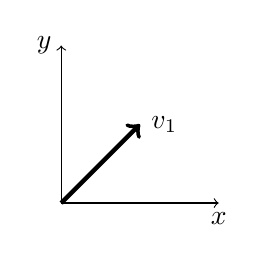
\begin{tikzpicture}
\def\v{2}
\def\x{1} % 2 * .5
\coordinate (O) at (0,0);
\coordinate (X) at (\x,\x);
\draw [->] (O) -- (\v,0) node[below]{$x$};
\draw [->] (O) -- (0,\v) node[left]{$y$};
\draw [ultra thick, ->] (O) -- (X) node[right]{$v_1$};
\end{tikzpicture}
\end{minipage}
\caption{Preference graph $G$, transition matrix $M$, and principal eigenvector $v_1$ for a two-node cycle. $||v_1||_2^2 = 1/2$, $H_T(G) = 1$. Intuitively, we set the probability of each item equal to the average of the prior preferences. The normalizing restriction on $v$ ensures that these averages continue to represent a distribution over the items. Note also that the steady state (a uniform distribution) is achieved after only one iteration.}
\label{fig:linalg_2} 
\end{figure}



\begin{figure}[!htb] % Three node transitive
\centering
\begin{minipage}{1.2in}
\begin{tikzpicture}[node distance=3cm]
\node [roundnode] (a) {a};
\node [roundnode] (b) [right of=a] {b};
\node [roundnode] (c) [below of=a] {c};
\draw[ultra thick, ->] (b) -- (a);
\draw[ultra thick, ->] (c) -- (b);
\draw[ultra thick, ->] (c) -- (a);
\end{tikzpicture}
\end{minipage}
\hfill
\begin{minipage}{1.2in}
\[
M=
  \begin{bmatrix}
    1 & 0 & 0 \\
    .5 & .5 & 0 \\
    .5 & .5 & 0
  \end{bmatrix}
\]
\end{minipage}
\hfill
\begin{minipage}{1.2in}
\begin{tikzpicture}
\def\v{2}
\def\x{2} % 2 * 1
\coordinate (O) at (0,0,0);
\coordinate (X) at (\x,0,0);
\draw [->] (O) -- (\v,0,0) node[below]{$x$};
\draw [->] (O) -- (0,\v,0) node[left]{$z$};
\draw [->] (O) -- (0,0,\v) node[below]{$y$};
\draw [ultra thick, ->] (O) -- (X) node[right]{$v_1$};
\end{tikzpicture}
\end{minipage}
\caption{Preference graph $G$, transition matrix $M$, and principal eigenvector $v_1$ for a three-node transitive preference. $||v_1||_2^2 = 1$, $H_T(G) = 0.918$. In this case, the steady state is achieved in the limit. At every iteration, C sends its probability mass to A and B evenly, and has no mass after the first iteration. B splits its mass between itself and A, while A directs all of its mass towards itself. The limiting convergence is due to the logarithmic reallocation of mass from B to A (a bit of a Zeno-style paradox).}
\label{fig:linalg_3} 
\end{figure}



\begin{figure}[!htb] % Three node cycle
\centering
\begin{minipage}{1.2in}
\begin{tikzpicture}[node distance=3cm]
\node [roundnode] (a) {a};
\node [roundnode] (b) [right of=a] {b};
\node [roundnode] (c) [below of=a] {c};
\draw[ultra thick, ->] (b) -- (a);
\draw[ultra thick, ->] (c) -- (b);
\draw[ultra thick, ->] (a) -- (c);
\end{tikzpicture}
\end{minipage}
\hfill
\begin{minipage}{1.2in}
\[
M=
  \begin{bmatrix}
    .5 & 0 & .5 \\
    .5 & .5 & 0 \\
    0 & .5 & .5
  \end{bmatrix}
\]
\end{minipage}
\hfill
\begin{minipage}{1.2in}
\begin{tikzpicture}
\def\v{2}
\def\x{.66} % 2 * 1/3
\coordinate (O) at (0,0,0);
\coordinate (X) at (\x,\x,\x);
\coordinate (Xxy) at (\x,0,\x);
\draw [->] (O) -- (\v,0,0) node[below]{$x$};
\draw [->] (O) -- (0,\v,0) node[left]{$z$};
\draw [->] (O) -- (0,0,\v) node[below]{$y$};
\draw [ultra thick, ->] (O) -- (X) node[right]{$v_1$};
\draw [dashed, color=red] (O) -- (Xxy);
\draw [dashed, color=red] (X) -- (Xxy);
\end{tikzpicture}
\end{minipage}
\caption{Preference graph $G$, transition matrix $M$, and principal eigenvector $v_1$ for a three-node cycle. $||v_1||_2^2 = 1/3$, $H_T(G) = 1.585$. Here the reallocation of probability mass across iterations exhibits more complex dynamics, and converges to $v_1$ in the limit.}
\label{fig:linalg_4} 
\end{figure}



\begin{figure}[!htb] % Three node double cycle
\centering
\begin{minipage}{1.2in}
\begin{tikzpicture}[node distance=3cm]
\node [roundnode] (a) {a};
\node [roundnode] (b) [right of=a] {b};
\node [roundnode] (c) [below of=a] {c};
\draw[ultra thick, ->] (b) to[bend right] (a);
\draw[ultra thick, ->] (c) to[bend right] (b);
\draw[ultra thick, ->] (a) to[bend right] (c);
\draw[ultra thick, ->] (a) -- (b);
\draw[ultra thick, ->] (b) -- (c);
\draw[ultra thick, ->] (c) -- (a);
\end{tikzpicture}
\end{minipage}
\hfill
\begin{minipage}{1.2in}
\[
M=
  \begin{bmatrix}
    .5 & .25 & .25 \\
    .25 & .5 & .25 \\
    .25 & .25 & .5
  \end{bmatrix}
\]
\end{minipage}
\hfill
\begin{minipage}{1.2in}
\begin{tikzpicture}
\def\v{2}
\def\x{.66} % 2 * 1/3
\coordinate (O) at (0,0,0);
\coordinate (X) at (\x,\x,\x);
\coordinate (Xxy) at (\x,0,\x);
\draw [->] (O) -- (\v,0,0) node[below]{$x$};
\draw [->] (O) -- (0,\v,0) node[left]{$z$};
\draw [->] (O) -- (0,0,\v) node[below]{$y$};
\draw [ultra thick, ->] (O) -- (X) node[right]{$v_1$};
\draw [dashed, color=red] (O) -- (Xxy);
\draw [dashed, color=red] (X) -- (Xxy);
\end{tikzpicture}
\end{minipage}
\caption{Preference graph $G$, transition matrix $M$, and principal eigenvector $v_1$ for a three-node double cycle. $||v_1||_2^2 = 1/3$, $H_T(G) = 1.585$}
\label{fig:linalg_5} 
\end{figure}



\begin{figure}[!htb] % Three node transitive with edge weights
\centering
\begin{minipage}{1.2in}
\begin{tikzpicture}[node distance=3cm]
\node [roundnode] (a) {a};
\node [roundnode] (b) [right of=a] {b};
\node [roundnode] (c) [below of=a] {c};
\draw[ultra thick, ->] (a) -- node[auto] {1} (b);
\draw[ultra thick, ->] (b) -- node[auto] {1} (c);
\draw[ultra thick, ->] (c) -- node[auto] {3} (a);
\end{tikzpicture}
\end{minipage}
\hfill
\begin{minipage}{1.2in}
\[
M=
  \begin{bmatrix}
    .75 & .25 & 0 \\
    0 & .5 & .5 \\
    .75 & 0 & .25
  \end{bmatrix}
\]
\end{minipage}
\hfill
\begin{minipage}{1.2in}
\begin{tikzpicture}
\def\v{2}
\def\a{1.09068489}
\def\b{0.54557228}
\def\c{0.36374283}
\coordinate (O) at (0,0,0);
\coordinate (X) at (\a,\c,\b);
\coordinate (Xxy) at (\a,0,\b);
\draw [->] (O) -- (\v,0,0) node[below]{$x$};
\draw [->] (O) -- (0,\v,0) node[left]{$z$};
\draw [->] (O) -- (0,0,\v) node[below]{$y$};
\draw [ultra thick, ->] (O) -- (X) node[right]{$v_1$};
\draw [dashed, color=red] (O) -- (Xxy);
\draw [dashed, color=red] (X) -- (Xxy);
\end{tikzpicture}
\end{minipage}
\caption{Preference graph $G$, transition matrix $M$, and principal eigenvector $v_1$ for a three-node cycle with edge weights. $||v_1||_2^2 = 0.4049$, $H_T(G) = 1.371$. Note how the introduction of variable weights repositions $v_1$ within the simplex, allowing us to recover a transitive ordering $a > b > c$.}
\label{fig:linalg_6} 
\end{figure}


\begin{figure}[!htb] % Four node two cycle
\centering
\begin{minipage}{1.2in}
\begin{tikzpicture}[node distance=3cm]
\node [roundnode] (a) {a};
\node [roundnode] (b) [right of=a] {b};
\node [roundnode] (c) [below of=a] {c};
\node [roundnode] (d) [below of=b] {d};
\draw[ultra thick, ->] (a) -- (c);
\draw[ultra thick, ->] (b) -- (a);
\draw[ultra thick, ->] (c) -- (b);
\draw[ultra thick, ->] (d) -- (a);
\draw[ultra thick, ->] (d) -- (b);
\draw[ultra thick, ->] (c) -- (d);
\end{tikzpicture}
\end{minipage}
\hfill
\begin{minipage}{1.2in}
\[
M=
  \begin{bmatrix}
    .66 & 0 & .33 & 0 \\
    .33 & .66 & 0 & 0 \\
    0 & .33 & .33 & .33 \\
    .33 & .33 & 0 & .33
  \end{bmatrix}
\]
\end{minipage}
\hfill
\begin{minipage}{1.2in}
\[
(.4, .3, .2, .1)
\]
\end{minipage}
\caption{Preference graph $G$, transition matrix $M$, and principal eigenvector $v_1$ for a four-node graph with two cycles. $||v_1||_2^2 = 0.3$, $H_T(G) = 1.918$.}
\label{fig:linalg_7} 
\end{figure}


\begin{figure}[!htb] % Four node upper cycle
\centering
\begin{minipage}{1.2in}
\begin{tikzpicture}[node distance=3cm]
\node [roundnode] (a) {a};
\node [roundnode] (b) [right of=a] {b};
\node [roundnode] (c) [below of=a] {c};
\node [roundnode] (d) [below of=b] {d};
\draw[ultra thick, ->] (a) -- (c);
\draw[ultra thick, ->] (c) -- (b);
\draw[ultra thick, ->] (b) -- (a);
\draw[ultra thick, ->] (d) -- (a);
\draw[ultra thick, ->] (d) -- (b);
\draw[ultra thick, ->] (d) -- (c);
\end{tikzpicture}
\end{minipage}
\hfill
\begin{minipage}{1.2in}
\[
M=
  \begin{bmatrix}
    .66 & 0 & .33 & 0 \\
    .33 & .66 & 0 & 0 \\
    0 & .33 & .66 & 0 \\
    .33 & .33 & .33 & 0
  \end{bmatrix}
\]
\end{minipage}
\hfill
\begin{minipage}{1.2in}
\[
(.33, .33, .33, 0)
\]
\end{minipage}
\caption{Preference graph $G$, transition matrix $M$, and principal eigenvector $v_1$ for a four-node graph with one cycle. $||v_1||_2^2 = 1/3$, $H_T(G) = 1.585$. Note that we see a cycle in $v_1$, despite having a larger $L_2$ value than the previous example.}
\label{fig:linalg_8} 
\end{figure}


\begin{figure}[!htb] % Four node lower cycle
\centering
\begin{minipage}{1.2in}
\begin{tikzpicture}[node distance=3cm]
\node [roundnode] (a) {a};
\node [roundnode] (b) [right of=a] {b};
\node [roundnode] (c) [below of=a] {c};
\node [roundnode] (d) [below of=b] {d};
\draw[ultra thick, ->] (b) -- (a);
\draw[ultra thick, ->] (c) -- (a);
\draw[ultra thick, ->] (d) -- (a);
\draw[ultra thick, ->] (b) -- (c);
\draw[ultra thick, ->] (c) -- (d);
\draw[ultra thick, ->] (d) -- (b);
\end{tikzpicture}
\end{minipage}
\hfill
\begin{minipage}{1.2in}
\[
M=
  \begin{bmatrix}
    1 & 0 & 0 & 0 \\
    .33 & .33 & .33 & 0 \\
    .33 & 0 & .33 & .33 \\
    .33 & .33 & 0 & .33
  \end{bmatrix}
\]
\end{minipage}
\hfill
\begin{minipage}{1.2in}
\[
(1, 0, 0, 0)
\]
\end{minipage}
\caption{Preference graph $G$, transition matrix $M$, and principal eigenvector $v_1$ for a four-node graph with one cycle. $||v_1||_2^2 = 1$, $H_T(G) = 1.793$. Note how the presence of a cycle in the lower nodes does not prevent the graph from having high level of structure.}
\label{fig:linalg_9} 
\end{figure}

% END LINALG FIGURES

This series of basic examples illustrate how the language of graphs and matrices allows us to make meaningful statements about preference in the presence of challenging structures like cycles, which manifest as contradictions when represented in terms of linear ordering.